\documentclass[]{article}
\usepackage{lmodern}
\usepackage{amssymb,amsmath}
\usepackage{ifxetex,ifluatex}
\usepackage{fixltx2e} % provides \textsubscript
\ifnum 0\ifxetex 1\fi\ifluatex 1\fi=0 % if pdftex
  \usepackage[T1]{fontenc}
  \usepackage[utf8]{inputenc}
\else % if luatex or xelatex
  \ifxetex
    \usepackage{mathspec}
  \else
    \usepackage{fontspec}
  \fi
  \defaultfontfeatures{Ligatures=TeX,Scale=MatchLowercase}
\fi
% use upquote if available, for straight quotes in verbatim environments
\IfFileExists{upquote.sty}{\usepackage{upquote}}{}
% use microtype if available
\IfFileExists{microtype.sty}{%
\usepackage{microtype}
\UseMicrotypeSet[protrusion]{basicmath} % disable protrusion for tt fonts
}{}
\usepackage[margin=1in]{geometry}
\usepackage{hyperref}
\hypersetup{unicode=true,
            pdftitle={Analysis of a genome annotation table},
            pdfauthor={Jacques van Helden},
            pdfborder={0 0 0},
            breaklinks=true}
\urlstyle{same}  % don't use monospace font for urls
\usepackage{color}
\usepackage{fancyvrb}
\newcommand{\VerbBar}{|}
\newcommand{\VERB}{\Verb[commandchars=\\\{\}]}
\DefineVerbatimEnvironment{Highlighting}{Verbatim}{commandchars=\\\{\}}
% Add ',fontsize=\small' for more characters per line
\usepackage{framed}
\definecolor{shadecolor}{RGB}{48,48,48}
\newenvironment{Shaded}{\begin{snugshade}}{\end{snugshade}}
\newcommand{\KeywordTok}[1]{\textcolor[rgb]{0.94,0.87,0.69}{#1}}
\newcommand{\DataTypeTok}[1]{\textcolor[rgb]{0.87,0.87,0.75}{#1}}
\newcommand{\DecValTok}[1]{\textcolor[rgb]{0.86,0.86,0.80}{#1}}
\newcommand{\BaseNTok}[1]{\textcolor[rgb]{0.86,0.64,0.64}{#1}}
\newcommand{\FloatTok}[1]{\textcolor[rgb]{0.75,0.75,0.82}{#1}}
\newcommand{\ConstantTok}[1]{\textcolor[rgb]{0.86,0.64,0.64}{\textbf{#1}}}
\newcommand{\CharTok}[1]{\textcolor[rgb]{0.86,0.64,0.64}{#1}}
\newcommand{\SpecialCharTok}[1]{\textcolor[rgb]{0.86,0.64,0.64}{#1}}
\newcommand{\StringTok}[1]{\textcolor[rgb]{0.80,0.58,0.58}{#1}}
\newcommand{\VerbatimStringTok}[1]{\textcolor[rgb]{0.80,0.58,0.58}{#1}}
\newcommand{\SpecialStringTok}[1]{\textcolor[rgb]{0.80,0.58,0.58}{#1}}
\newcommand{\ImportTok}[1]{\textcolor[rgb]{0.80,0.80,0.80}{#1}}
\newcommand{\CommentTok}[1]{\textcolor[rgb]{0.50,0.62,0.50}{#1}}
\newcommand{\DocumentationTok}[1]{\textcolor[rgb]{0.50,0.62,0.50}{#1}}
\newcommand{\AnnotationTok}[1]{\textcolor[rgb]{0.50,0.62,0.50}{\textbf{#1}}}
\newcommand{\CommentVarTok}[1]{\textcolor[rgb]{0.50,0.62,0.50}{\textbf{#1}}}
\newcommand{\OtherTok}[1]{\textcolor[rgb]{0.94,0.94,0.56}{#1}}
\newcommand{\FunctionTok}[1]{\textcolor[rgb]{0.94,0.94,0.56}{#1}}
\newcommand{\VariableTok}[1]{\textcolor[rgb]{0.80,0.80,0.80}{#1}}
\newcommand{\ControlFlowTok}[1]{\textcolor[rgb]{0.94,0.87,0.69}{#1}}
\newcommand{\OperatorTok}[1]{\textcolor[rgb]{0.94,0.94,0.82}{#1}}
\newcommand{\BuiltInTok}[1]{\textcolor[rgb]{0.80,0.80,0.80}{#1}}
\newcommand{\ExtensionTok}[1]{\textcolor[rgb]{0.80,0.80,0.80}{#1}}
\newcommand{\PreprocessorTok}[1]{\textcolor[rgb]{1.00,0.81,0.69}{\textbf{#1}}}
\newcommand{\AttributeTok}[1]{\textcolor[rgb]{0.80,0.80,0.80}{#1}}
\newcommand{\RegionMarkerTok}[1]{\textcolor[rgb]{0.80,0.80,0.80}{#1}}
\newcommand{\InformationTok}[1]{\textcolor[rgb]{0.50,0.62,0.50}{\textbf{#1}}}
\newcommand{\WarningTok}[1]{\textcolor[rgb]{0.50,0.62,0.50}{\textbf{#1}}}
\newcommand{\AlertTok}[1]{\textcolor[rgb]{1.00,0.81,0.69}{#1}}
\newcommand{\ErrorTok}[1]{\textcolor[rgb]{0.76,0.75,0.62}{#1}}
\newcommand{\NormalTok}[1]{\textcolor[rgb]{0.80,0.80,0.80}{#1}}
\usepackage{longtable,booktabs}
\usepackage{graphicx,grffile}
\makeatletter
\def\maxwidth{\ifdim\Gin@nat@width>\linewidth\linewidth\else\Gin@nat@width\fi}
\def\maxheight{\ifdim\Gin@nat@height>\textheight\textheight\else\Gin@nat@height\fi}
\makeatother
% Scale images if necessary, so that they will not overflow the page
% margins by default, and it is still possible to overwrite the defaults
% using explicit options in \includegraphics[width, height, ...]{}
\setkeys{Gin}{width=\maxwidth,height=\maxheight,keepaspectratio}
\IfFileExists{parskip.sty}{%
\usepackage{parskip}
}{% else
\setlength{\parindent}{0pt}
\setlength{\parskip}{6pt plus 2pt minus 1pt}
}
\setlength{\emergencystretch}{3em}  % prevent overfull lines
\providecommand{\tightlist}{%
  \setlength{\itemsep}{0pt}\setlength{\parskip}{0pt}}
\setcounter{secnumdepth}{0}
% Redefines (sub)paragraphs to behave more like sections
\ifx\paragraph\undefined\else
\let\oldparagraph\paragraph
\renewcommand{\paragraph}[1]{\oldparagraph{#1}\mbox{}}
\fi
\ifx\subparagraph\undefined\else
\let\oldsubparagraph\subparagraph
\renewcommand{\subparagraph}[1]{\oldsubparagraph{#1}\mbox{}}
\fi

%%% Use protect on footnotes to avoid problems with footnotes in titles
\let\rmarkdownfootnote\footnote%
\def\footnote{\protect\rmarkdownfootnote}

%%% Change title format to be more compact
\usepackage{titling}

% Create subtitle command for use in maketitle
\providecommand{\subtitle}[1]{
  \posttitle{
    \begin{center}\large#1\end{center}
    }
}

\setlength{\droptitle}{-2em}

  \title{Analysis of a genome annotation table}
    \pretitle{\vspace{\droptitle}\centering\huge}
  \posttitle{\par}
  \subtitle{Probabilités et statistique pour la biologie (STAT1)}
  \author{Jacques van Helden}
    \preauthor{\centering\large\emph}
  \postauthor{\par}
      \predate{\centering\large\emph}
  \postdate{\par}
    \date{2019-09-19}


\begin{document}
\maketitle

{
\setcounter{tocdepth}{3}
\tableofcontents
}
\subsection{Goal of this practical}\label{goal-of-this-practical}

During this practical session, you will run the following tasks:

\begin{enumerate}
\def\labelenumi{\arabic{enumi}.}
\tightlist
\item
  Handle a table containing annotated features of the yeast genome.
\item
  Select a subset of the data by filtering rows based on a given
  criterion (annotation type, chromosome, \ldots{})
\item
  Generate graphics to represent different aspects of the data.
\item
  Compute estimators of central tendency and dispersion.
\item
  Compute a confidence interval around the mean.
\end{enumerate}

\subsection{Expected report}\label{expected-report}

At the end of the practical you will be asked to submit two documents

\begin{enumerate}
\def\labelenumi{\arabic{enumi}.}
\tightlist
\item
  Your \textbf{R code}.Each question must be explicitly formulated
  before presenting the results that answer it and giving an
  interpretation of these results.
\item
  UA \textbf{synthetic report}, which will include a presentation of the
  main results (figures, descriptives stats, tables) as well as your
  interpretation of the result.
\end{enumerate}

\subsubsection{Expectation for the code}\label{expectation-for-the-code}

\begin{enumerate}
\def\labelenumi{\arabic{enumi}.}
\item
  The code must be \textbf{readable and undestandable}: choose variable
  names that explicitly indicate what they represent.
\item
  The code must be properly documented (the \texttt{\#} symbol starts a
  comment, either at the begining or in the middle of a line of code).

  \begin{itemize}
  \item
    Before each chunk of code, explain what this code is supposed to do,
    what it serves to.
  \item
    Don't hesitate to occasionally add some comment words to justify the
    chosen approach.
  \item
    Each time you define a variable, add a comment on the same line to
    indicate what this variable represents.
  \end{itemize}
\item
  The code must be \textbf{portable}: other people should be able to
  download it and run it on their computer. For this practical, I will
  systematically test whether your code can run on my computer.
  hard-coded absolute paths of a file on your machine should thus always
  be avoided (we will indicate hereafter how to define relative paths
  relative to the root of your user account).
\end{enumerate}

\subsubsection{Expected content for the interpretation
report}\label{expected-content-for-the-interpretation-report}

Your report must be synthetic (1 text page max + as many figures and
table as you wish) Le rapport doit être synthétique (1 page de texte
maximum + autant de figures et tables que vous le désirez).

Each question must be explicitly formulated before presenting the
results that answer it and then interpreting those results.\\
Chaque question doit être exprimée explicitement avant de présenter les
résultats qui y répondent et de fournir l'interprétation de ces
résultats.

Each figure or table must be documented with a legend that allows a
naive reader to understand what it represents. The interpretation of the
results displayed on a figure or table will be found in the main text
(with a reference to the figure or table number). Chaque figure ou table
doit être documentée par une légende permettant à un lecteur naïf de
comprendre ce qu'elle représente. L'interprétation des résultats
affichés sur une figure ou table se trouvera dans le texte principal
(avec une référence au numéro de figure ou table).

\subsection{Historical example: yeast
genome}\label{historical-example-yeast-genome}

\begin{itemize}
\tightlist
\item
  1992: publication of the first complete eukaryotic chromosome, the 3rd
  yeast chromosome.
\item
  1996: publication of the complete genome.
\end{itemize}

On the base of the genes of the 3rd chromosome (sample) we can estimate
the average size of a yeast gene.

\textbf{Questions: }

\begin{enumerate}
\def\labelenumi{(\alph{enumi})}
\item
  Would the sample mean (chromosome III) be sufficient to predict the
  population mean (complete genome)~?

  To answer this question, we will imagine that we came back in 1992,
  and will use all the genes of chromosome III (considered here as a
  sample of the genome) to estimate the average size of genes for the
  whole genome (the ``population'' of genes``).
\item
  Can this sample be described as ``simple and independent''~?
\end{enumerate}

\subsection{Analysis of the length of the baker's yeast
genes}\label{analysis-of-the-length-of-the-bakers-yeast-genes}

\begin{figure}

{\centering 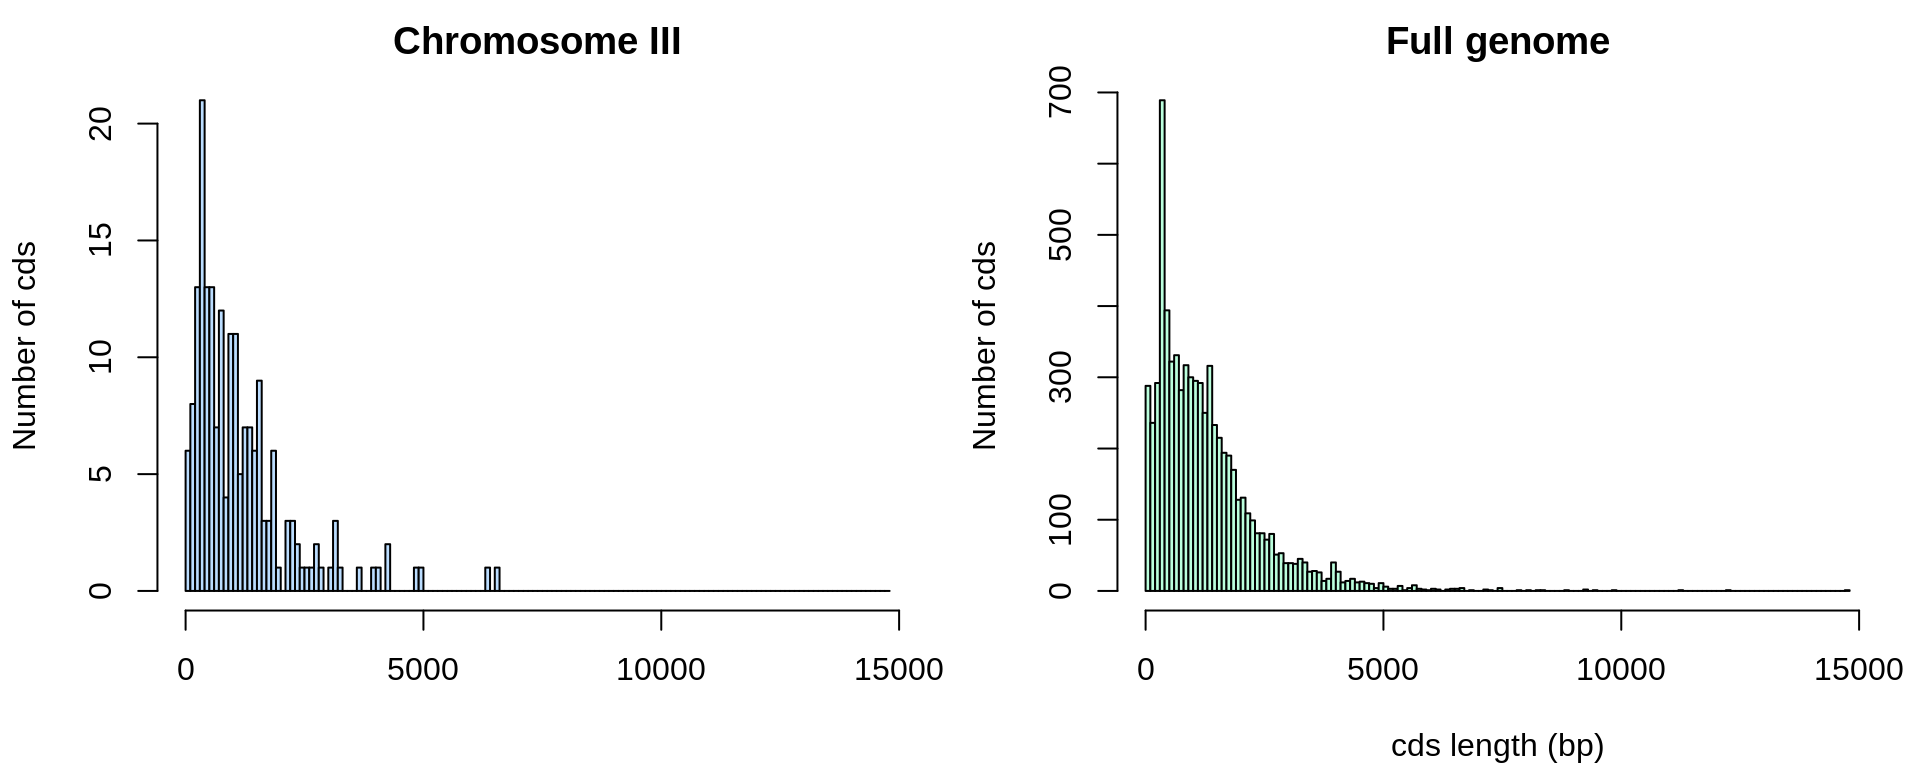
\includegraphics[width=0.9\linewidth]{figures/cds_length_histo-1} 

}

\caption{Distribution of cds lengths for Saccharomyces cerevisiae. }\label{fig:cds_length_histo}
\end{figure}

\subsection{Tutorial}\label{tutorial}

Before moving to the exercises, we show you here some basic elements
about reading, manipulating and writing data tables with R.

\subsubsection{The path to the home
(manual)}\label{the-path-to-the-home-manual}

We will create a folder for this tutorial, starting from the root of our
account.

First possibility (\textbf{quick but not very elegant}): enter
(manually) the path from the root of your account in a variable

\texttt{dir.home\ \textless{}-\ /the/path/to/the/home}

\begin{itemize}
\tightlist
\item
  Advantage: fast and convenient
\item
  Disadvantage: not portable, will only work on your computer
\end{itemize}

\subsubsection{The path to the home
(automatic)}\label{the-path-to-the-home-automatic}

A more general solution: use the \textbf{R} command
\texttt{Sys.getenv()}.

\begin{itemize}
\tightlist
\item
  Invoked without parameters, this command lists all environment
  variables (your system configuration).
\item
  The output can be restricted to a given environment variable, for
  example \texttt{Sys.getenv("HOME")} returns the path to the root of
  your account.
\end{itemize}

\textbf{Note:} equivalent writing with Linux: the tilde symbol
\texttt{\textasciitilde{}} also indicates the path to the root of your
account.

\begin{Shaded}
\begin{Highlighting}[]
\NormalTok{## Identify the home directory }
\NormalTok{## by getting the environment variable HOME }
\NormalTok{dir.home <-}\StringTok{ }\KeywordTok{Sys.getenv}\NormalTok{(}\StringTok{"HOME"}\NormalTok{)}
\KeywordTok{print}\NormalTok{(dir.home)}
\end{Highlighting}
\end{Shaded}

\begin{verbatim}
[1] "/home/khamvongsa"
\end{verbatim}

\subsubsection{Creating a folder for the
TP}\label{creating-a-folder-for-the-tp}

\begin{Shaded}
\begin{Highlighting}[]
\NormalTok{## Define a variable containing the path of the results for this tutorial}
\NormalTok{dir.tuto <-}\StringTok{ }\KeywordTok{file.path}\NormalTok{(dir.home, }\StringTok{"stat1"}\NormalTok{, }\StringTok{"TP2"}\NormalTok{)}

\KeywordTok{print}\NormalTok{(dir.tuto)}
\end{Highlighting}
\end{Shaded}

\begin{verbatim}
[1] "/home/khamvongsa/stat1/TP2"
\end{verbatim}

\begin{Shaded}
\begin{Highlighting}[]
\NormalTok{## Create the directory for this tutorial}
\KeywordTok{dir.create}\NormalTok{(}\DataTypeTok{path =}\NormalTok{ dir.tuto, }\DataTypeTok{showWarnings =} \OtherTok{FALSE}\NormalTok{, }\DataTypeTok{recursive =} \OtherTok{TRUE}\NormalTok{)}

\NormalTok{## Go to the tutorial directory}
\KeywordTok{setwd}\NormalTok{(dir.tuto)}

\NormalTok{## List the files already present in the folder (if any)}
\KeywordTok{list.files}\NormalTok{()}
\end{Highlighting}
\end{Shaded}

\begin{verbatim}
character(0)
\end{verbatim}

\subsubsection{Downloading the GTF file from
EnsemblGenomes}\label{downloading-the-gtf-file-from-ensemblgenomes}

\textbf{Tips: } before downloading the annotation file (GTF) from
EnsemblGenomes to our computer, we will check if it is already present
(and in this case we do not re-download it).

\begin{Shaded}
\begin{Highlighting}[]
\NormalTok{## Define the URL of the annotation file (GTF-formatted)}
\NormalTok{gtf.URL <-}\StringTok{ "ftp://ftp.ensemblgenomes.org/pub/release-37/fungi/gtf/saccharomyces_cerevisiae/Saccharomyces_cerevisiae.R64-1-1.37.gtf.gz"}

\NormalTok{## Define the path where the local copy will be stored}
\NormalTok{local.GTF <-}\StringTok{ }\KeywordTok{file.path}\NormalTok{(dir.tuto, }\StringTok{"Saccharomyces_cerevisiae.R64-1-1.37.gtf.gz"}\NormalTok{)}

\NormalTok{## If the local file file laready exists, skip the download}
\ControlFlowTok{if}\NormalTok{ (}\KeywordTok{file.exists}\NormalTok{(local.GTF)) \{}
  \KeywordTok{message}\NormalTok{(}\StringTok{"GTF file already exists in the tutorial folder: "}\NormalTok{, local.GTF)}
\NormalTok{\} }\ControlFlowTok{else}\NormalTok{ \{}
\NormalTok{  ## Download annotation table in GTF format}
  \KeywordTok{download.file}\NormalTok{(}\DataTypeTok{url =}\NormalTok{ gtf.URL, }\DataTypeTok{destfile =}\NormalTok{ local.GTF)}
\NormalTok{\}}
\end{Highlighting}
\end{Shaded}

\subsubsection{Loading a data table}\label{loading-a-data-table}

R has several types of tabular structures (matrix, data.frame, table).

The most commonly used structure is the \texttt{data.frame}, which
consists of an array of values (numeric or strings) whose rows and
columns are associated with names.

The function \texttt{read.table()} allows you to read a text file
containing a data table, and store the content in a variable.

Several functions derived from \texttt{read.table()} make it easier to
read different types of formats:

\begin{itemize}
\tightlist
\item
  \texttt{read.delim()} for files whose columns are delimited by a
  particular character (usually the tab, represented by ``\t'').
\item
  \texttt{read.csv()} for files ``comma-searated values''.
\end{itemize}

\begin{enumerate}
\def\labelenumi{\arabic{enumi}.}
\tightlist
\item
  Download the following file to your computer:
\end{enumerate}

\begin{itemize}
\tightlist
\item
  \href{../../data/Saccharomyces_cerevisiae/Saccharomyces_cerevisiae.R64-1-1.37.gtf}{Saccharomyces\_cerevisiae.R64-1-1.37.gtf}
\end{itemize}

\begin{enumerate}
\def\labelenumi{\arabic{enumi}.}
\setcounter{enumi}{1}
\tightlist
\item
  Load it using the read.table function (for this you must replace the
  path below by that of your computer).
\end{enumerate}

\begin{Shaded}
\begin{Highlighting}[]
\NormalTok{## Read a GTF file with yeast genome annotations}

\NormalTok{## Load the feature table}
\NormalTok{feature.table <-}\StringTok{ }\KeywordTok{read.table}\NormalTok{(}
\NormalTok{  local.GTF, }
  \DataTypeTok{comment.char =} \StringTok{"#"}\NormalTok{, }
  \DataTypeTok{sep=}\StringTok{"}\CharTok{\textbackslash{}t}\StringTok{"}\NormalTok{, }
  \DataTypeTok{header=}\OtherTok{FALSE}\NormalTok{, }
  \DataTypeTok{row.names=}\OtherTok{NULL}\NormalTok{)}

\NormalTok{## The bed format does not contain any column header, }
\NormalTok{## so we set it manually based on the description of the format, }
\NormalTok{## found here: }
\NormalTok{##     http://www.ensembl.org/info/website/upload/gff.html}
\KeywordTok{names}\NormalTok{(feature.table) <-}\StringTok{ }\KeywordTok{c}\NormalTok{(}\StringTok{"seqname"}\NormalTok{, }\StringTok{"source"}\NormalTok{, }\StringTok{"feature"}\NormalTok{, }\StringTok{"start"}\NormalTok{, }\StringTok{"end"}\NormalTok{, }\StringTok{"score"}\NormalTok{, }\StringTok{"strand"}\NormalTok{, }\StringTok{"frame"}\NormalTok{, }\StringTok{"attribute"}\NormalTok{)}
\end{Highlighting}
\end{Shaded}

\subsubsection{Exploring the content of a data
table}\label{exploring-the-content-of-a-data-table}

The first thing to do after loading a data table is to check its
dimensions.

\begin{Shaded}
\begin{Highlighting}[]
\KeywordTok{dim}\NormalTok{(feature.table) ## Dimensions of the tbale}
\end{Highlighting}
\end{Shaded}

\begin{verbatim}
[1] 43028     9
\end{verbatim}

\begin{Shaded}
\begin{Highlighting}[]
\KeywordTok{nrow}\NormalTok{(feature.table) ## Number of rows}
\end{Highlighting}
\end{Shaded}

\begin{verbatim}
[1] 43028
\end{verbatim}

\begin{Shaded}
\begin{Highlighting}[]
\KeywordTok{ncol}\NormalTok{(feature.table) ## Number of columns}
\end{Highlighting}
\end{Shaded}

\begin{verbatim}
[1] 9
\end{verbatim}

The display of the complete annotation table would not be very readable,
since it contains tens of thousands of lines.

We can display the first lines with the function \texttt{head()}.

\textbf{Note: } the last column is particularly heavy (it contains a lot
of information). We will see later how to select a subset of the columns
to simplify the display.

\begin{Shaded}
\begin{Highlighting}[]
\NormalTok{## Display the 5 first rows of the feature table}
\KeywordTok{head}\NormalTok{(feature.table, }\DataTypeTok{n =} \DecValTok{5}\NormalTok{) }
\end{Highlighting}
\end{Shaded}

\begin{verbatim}
  seqname source     feature start  end score strand frame
1      IV    SGD        gene  1802 2953     .      +     .
2      IV    SGD  transcript  1802 2953     .      +     .
3      IV    SGD        exon  1802 2953     .      +     .
4      IV    SGD         CDS  1802 2950     .      +     0
5      IV    SGD start_codon  1802 1804     .      +     0
                                                                                                                                                                                                                                    attribute
1                                                                                                                                                              gene_id YDL248W; gene_name COS7; gene_source SGD; gene_biotype protein_coding;
2                                                       gene_id YDL248W; transcript_id YDL248W; gene_name COS7; gene_source SGD; gene_biotype protein_coding; transcript_name COS7; transcript_source SGD; transcript_biotype protein_coding;
3                     gene_id YDL248W; transcript_id YDL248W; exon_number 1; gene_name COS7; gene_source SGD; gene_biotype protein_coding; transcript_name COS7; transcript_source SGD; transcript_biotype protein_coding; exon_id YDL248W.1;
4 gene_id YDL248W; transcript_id YDL248W; exon_number 1; gene_name COS7; gene_source SGD; gene_biotype protein_coding; transcript_name COS7; transcript_source SGD; transcript_biotype protein_coding; protein_id YDL248W; protein_version 1;
5                                        gene_id YDL248W; transcript_id YDL248W; exon_number 1; gene_name COS7; gene_source SGD; gene_biotype protein_coding; transcript_name COS7; transcript_source SGD; transcript_biotype protein_coding;
\end{verbatim}

The function \texttt{tail()} displays the last few lines:

\begin{Shaded}
\begin{Highlighting}[]
\NormalTok{## Display the 5 last rows of the feature table}
\KeywordTok{tail}\NormalTok{(feature.table, }\DataTypeTok{n =} \DecValTok{5}\NormalTok{) }
\end{Highlighting}
\end{Shaded}

\begin{verbatim}
      seqname source     feature start   end score strand frame
43024    Mito    SGD  transcript 85554 85709     .      +     .
43025    Mito    SGD        exon 85554 85709     .      +     .
43026    Mito    SGD         CDS 85554 85706     .      +     0
43027    Mito    SGD start_codon 85554 85556     .      +     0
43028    Mito    SGD  stop_codon 85707 85709     .      +     0
                                                                                                                                                                                            attribute
43024                                                     gene_id Q0297; transcript_id Q0297; gene_source SGD; gene_biotype protein_coding; transcript_source SGD; transcript_biotype protein_coding;
43025                     gene_id Q0297; transcript_id Q0297; exon_number 1; gene_source SGD; gene_biotype protein_coding; transcript_source SGD; transcript_biotype protein_coding; exon_id Q0297.1;
43026 gene_id Q0297; transcript_id Q0297; exon_number 1; gene_source SGD; gene_biotype protein_coding; transcript_source SGD; transcript_biotype protein_coding; protein_id Q0297; protein_version 1;
43027                                      gene_id Q0297; transcript_id Q0297; exon_number 1; gene_source SGD; gene_biotype protein_coding; transcript_source SGD; transcript_biotype protein_coding;
43028                                      gene_id Q0297; transcript_id Q0297; exon_number 1; gene_source SGD; gene_biotype protein_coding; transcript_source SGD; transcript_biotype protein_coding;
\end{verbatim}

If you are using the \textbf{RStudio} environment, you can display the
table in a dynamic viewer pane with the function \texttt{View()}.

\begin{Shaded}
\begin{Highlighting}[]
\NormalTok{## In RStudio, display the table in a separate tab}
\KeywordTok{View}\NormalTok{(feature.table) }
\end{Highlighting}
\end{Shaded}

\subsubsection{Selection of subsets from a
table}\label{selection-of-subsets-from-a-table}

Selection of a line specified by its index.

\begin{Shaded}
\begin{Highlighting}[]
\NormalTok{feature.table[}\DecValTok{12}\NormalTok{,]}
\end{Highlighting}
\end{Shaded}

\begin{verbatim}
   seqname source    feature start  end score strand frame
12      IV    SGD stop_codon  3834 3836     .      +     0
                                                                                                                                                            attribute
12 gene_id YDL247W-A; transcript_id YDL247W-A; exon_number 1; gene_source SGD; gene_biotype protein_coding; transcript_source SGD; transcript_biotype protein_coding;
\end{verbatim}

Selection of a column specified by its index (display of the first
values only).

\begin{Shaded}
\begin{Highlighting}[]
\KeywordTok{head}\NormalTok{(feature.table[,}\DecValTok{3}\NormalTok{])}
\end{Highlighting}
\end{Shaded}

\begin{verbatim}
[1] gene        transcript  exon        CDS         start_codon stop_codon 
Levels: CDS exon gene start_codon stop_codon transcript
\end{verbatim}

Selection of a cell by combining row and column indices.

\begin{Shaded}
\begin{Highlighting}[]
\NormalTok{feature.table[}\DecValTok{12}\NormalTok{, }\DecValTok{3}\NormalTok{]}
\end{Highlighting}
\end{Shaded}

\begin{verbatim}
[1] stop_codon
Levels: CDS exon gene start_codon stop_codon transcript
\end{verbatim}

Selection of a column and/or row set.

\begin{Shaded}
\begin{Highlighting}[]
\NormalTok{feature.table[}\DecValTok{100}\OperatorTok{:}\DecValTok{105}\NormalTok{, }\DecValTok{1}\OperatorTok{:}\DecValTok{6}\NormalTok{]}
\end{Highlighting}
\end{Shaded}

\begin{verbatim}
    seqname source     feature start   end score
100      IV    SGD         CDS 34240 36477     .
101      IV    SGD start_codon 36475 36477     .
102      IV    SGD  stop_codon 34237 34239     .
103      IV    SGD        gene 36797 38173     .
104      IV    SGD  transcript 36797 38173     .
105      IV    SGD        exon 36797 38173     .
\end{verbatim}

Selection of specific columns (here, the genomic coordinates of each
feature): chromosome, beginning, end, strand.

\begin{Shaded}
\begin{Highlighting}[]
\NormalTok{feature.table[}\DecValTok{100}\OperatorTok{:}\DecValTok{105}\NormalTok{, }\KeywordTok{c}\NormalTok{(}\DecValTok{1}\NormalTok{,}\DecValTok{4}\NormalTok{,}\DecValTok{5}\NormalTok{,}\DecValTok{7}\NormalTok{)]}
\end{Highlighting}
\end{Shaded}

\begin{verbatim}
    seqname start   end strand
100      IV 34240 36477      -
101      IV 36475 36477      -
102      IV 34237 34239      -
103      IV 36797 38173      +
104      IV 36797 38173      +
105      IV 36797 38173      +
\end{verbatim}

Select a column based on its name.

\begin{Shaded}
\begin{Highlighting}[]
\NormalTok{## Select the "start" column and print the 100 first results}
\KeywordTok{head}\NormalTok{(feature.table}\OperatorTok{$}\NormalTok{start, }\DataTypeTok{n=}\DecValTok{100}\NormalTok{)}
\end{Highlighting}
\end{Shaded}

\begin{verbatim}
  [1]  1802  1802  1802  1802  1802  2951  3762  3762  3762  3762  3762
 [12]  3834  5985  5985  5985  5985  5985  7812  8683  8683  8683  8686
 [23]  9754  8683 11657 11657 11657 11660 13358 11657 16204 16204 16204
 [34] 16204 16204 17224 17577 17577 17577 17580 18564 17577 18959 18959
 [45] 18959 18959 18959 19310 20635 20635 20635 20635 20635 21004 22471
 [56] 22471 22471 22474 22606 22471 22823 22823 22823 22823 22823 25874
 [67] 26403 26403 26403 26406 28773 26403 28985 28985 28985 28988 30452
 [78] 28985 30657 30657 30657 30657 30657 31827 32296 32296 32296 32296
 [89] 32296 33232 33415 33415 33415 33418 33916 33415 34237 34237 34237
[100] 34240
\end{verbatim}

\begin{Shaded}
\begin{Highlighting}[]
\NormalTok{## Print the 20 first values of the "feature" field, which indicates the feature type}
\KeywordTok{head}\NormalTok{(feature.table}\OperatorTok{$}\NormalTok{feature, }\DataTypeTok{n=}\DecValTok{20}\NormalTok{)}
\end{Highlighting}
\end{Shaded}

\begin{verbatim}
 [1] gene        transcript  exon        CDS         start_codon
 [6] stop_codon  gene        transcript  exon        CDS        
[11] start_codon stop_codon  gene        transcript  exon       
[16] CDS         start_codon stop_codon  gene        transcript 
Levels: CDS exon gene start_codon stop_codon transcript
\end{verbatim}

Selection of several columns based on their names.

\begin{Shaded}
\begin{Highlighting}[]
\NormalTok{## Select the "start" column and print the 100 first results}
\NormalTok{feature.table[}\DecValTok{100}\OperatorTok{:}\DecValTok{106}\NormalTok{, }\KeywordTok{c}\NormalTok{(}\StringTok{"seqname"}\NormalTok{, }\StringTok{"start"}\NormalTok{, }\StringTok{"end"}\NormalTok{, }\StringTok{"strand"}\NormalTok{)]}
\end{Highlighting}
\end{Shaded}

\begin{verbatim}
    seqname start   end strand
100      IV 34240 36477      -
101      IV 36475 36477      -
102      IV 34237 34239      -
103      IV 36797 38173      +
104      IV 36797 38173      +
105      IV 36797 38173      +
106      IV 36797 38170      +
\end{verbatim}

\textbf{Note}: Selection of several columns based on their names. It is
also possible to name the rows of a data.frame but the GTF table does
not support this. We will see more examples later.

\subsubsection{Selection of a subset of rows based on the content of a
column}\label{selection-of-a-subset-of-rows-based-on-the-content-of-a-column}

The function \texttt{subset()} allows you to select a subset of the rows
of a data.frame based on a condition applied to one or more columns.

We can apply it to select the subset of rows in the annotation table
corresponding to coding sequences (CDS).

\begin{Shaded}
\begin{Highlighting}[]
\NormalTok{## Select subset of features having "cds" as "feature" attribute}
\NormalTok{cds <-}\StringTok{ }\KeywordTok{subset}\NormalTok{(feature.table, feature}\OperatorTok{==}\StringTok{"cds"}\NormalTok{)}

\KeywordTok{nrow}\NormalTok{(feature.table) ## Count the number of features}
\end{Highlighting}
\end{Shaded}

\begin{verbatim}
[1] 43028
\end{verbatim}

\begin{Shaded}
\begin{Highlighting}[]
\KeywordTok{nrow}\NormalTok{(cds) ## Count the number of cds}
\end{Highlighting}
\end{Shaded}

\begin{verbatim}
[1] 0
\end{verbatim}

\subsubsection{Count by value}\label{count-by-value}

The function \texttt{table()} allows you to count the occurrences of
each value in a vector or array. Some examples of use below.

\begin{Shaded}
\begin{Highlighting}[]
\NormalTok{## Count the number of featues per chromosome}
\KeywordTok{table}\NormalTok{(feature.table}\OperatorTok{$}\NormalTok{seqname)}
\end{Highlighting}
\end{Shaded}

\begin{verbatim}

   I   II  III   IV   IX Mito    V   VI  VII VIII    X   XI  XII XIII  XIV 
 759 2912 1210 5374 1567  327 2159  946 3856 2054 2617 2231 3789 3311 2774 
  XV  XVI 
3846 3296 
\end{verbatim}

\begin{Shaded}
\begin{Highlighting}[]
\NormalTok{## Count the number of features per type}
\KeywordTok{table}\NormalTok{(feature.table}\OperatorTok{$}\NormalTok{feature)}
\end{Highlighting}
\end{Shaded}

\begin{verbatim}

        CDS        exon        gene start_codon  stop_codon  transcript 
       7050        7872        7445        6700        6516        7445 
\end{verbatim}

Contingency tables can be calculated by counting the number of
combinations between 2 vectors (or 2 columns of a table).

\begin{Shaded}
\begin{Highlighting}[]
\NormalTok{##  Table with two vectors}
\KeywordTok{table}\NormalTok{(feature.table}\OperatorTok{$}\NormalTok{feature, feature.table}\OperatorTok{$}\NormalTok{seqname)}
\end{Highlighting}
\end{Shaded}

\begin{verbatim}
             
                I  II III  IV  IX Mito   V  VI VII VIII   X  XI XII XIII
  CDS         122 492 194 895 255   59 345 151 619  346 422 361 615  544
  exon        137 525 224 961 288   94 400 180 710  373 480 404 698  610
  gene        132 494 213 914 274   62 383 167 676  349 458 388 658  573
  start_codon 119 464 185 853 243   28 328 143 593  325 406 348 586  514
  stop_codon  117 443 181 837 233   22 320 138 582  312 393 342 574  497
  transcript  132 494 213 914 274   62 383 167 676  349 458 388 658  573
             
              XIV  XV XVI
  CDS         458 623 549
  exon        500 689 599
  gene        475 665 564
  start_codon 438 607 520
  stop_codon  428 597 500
  transcript  475 665 564
\end{verbatim}

\begin{Shaded}
\begin{Highlighting}[]
\NormalTok{## Same result with a 2-column data frame}
\KeywordTok{table}\NormalTok{(feature.table[, }\KeywordTok{c}\NormalTok{(}\StringTok{"feature"}\NormalTok{, }\StringTok{"seqname"}\NormalTok{)])}
\end{Highlighting}
\end{Shaded}

\begin{verbatim}
             seqname
feature         I  II III  IV  IX Mito   V  VI VII VIII   X  XI XII XIII
  CDS         122 492 194 895 255   59 345 151 619  346 422 361 615  544
  exon        137 525 224 961 288   94 400 180 710  373 480 404 698  610
  gene        132 494 213 914 274   62 383 167 676  349 458 388 658  573
  start_codon 119 464 185 853 243   28 328 143 593  325 406 348 586  514
  stop_codon  117 443 181 837 233   22 320 138 582  312 393 342 574  497
  transcript  132 494 213 914 274   62 383 167 676  349 458 388 658  573
             seqname
feature       XIV  XV XVI
  CDS         458 623 549
  exon        500 689 599
  gene        475 665 564
  start_codon 438 607 520
  stop_codon  428 597 500
  transcript  475 665 564
\end{verbatim}

\subsection{Exercises}\label{exercises}

\subsubsection{1. GTF format
specifications}\label{gtf-format-specifications}

Read the GTF format specifications.

\begin{itemize}
\tightlist
\item
  Ensembl (\url{http://www.ensembl.org/info/website/upload/gff.html})
\item
  UCSC (\url{https://genome.ucsc.edu/FAQ/FAQformat.html\#format4})
\end{itemize}

\subsubsection{2. Creating a local folder for the
TP}\label{creating-a-local-folder-for-the-tp}

Create a local folder (for example: \texttt{stat1/TP\_yeast} from the
root of your account). We suggest you to use the following functions:

\begin{itemize}
\tightlist
\item
  \texttt{Sys.getenv("HOME")} (Linnux and Mac OS X), to get the root of
  your user account;
\item
  \texttt{file.path()} to build a path;
\item
  \texttt{dir.create()} to create the folder for the TP. Read carefully
  the options of this function with \texttt{help(dir.create)}
\end{itemize}

\subsubsection{3. Locating the annotation
file}\label{locating-the-annotation-file}

Locate the yeast genome annotation file in GTF format in this local
folder.

\begin{itemize}
\tightlist
\item
  Site Ensembl Fungi: \url{http://fungi.ensembl.org/}
\item
  Click ``Downloads'' to access the
  \href{http://fungi.ensembl.org/info/website/ftp/}{ftp website}
\item
  In the search box, type \emph{``saccharomyces cerevisiae''} and follow
  the link
  ``\href{ftp://ftp.ensemblgenomes.org/pub/release-37/fungi/gtf/saccharomyces_cerevisiae}{GTF}''
\item
  Copy the address (URL) of the file
  \href{ftp://ftp.ensemblgenomes.org/pub/release-37/fungi/gtf/saccharomyces_cerevisiae/Saccharomyces_cerevisiae.R64-1-1.37.gtf.gz}{Saccharomyces\_cerevisiae.R64-1-1.37.gtf.gz}
\end{itemize}

\subsubsection{4. Downloading a file from an ftp
site}\label{downloading-a-file-from-an-ftp-site}

Suggested functions:

\begin{itemize}
\tightlist
\item
  \texttt{download.file()} (read the help to know the arguments)
\end{itemize}

\subsubsection{5. Loading a data table in
R}\label{loading-a-data-table-in-r}

Write a script that loads the data table into a variable named
\texttt{feature.table}, using the function R \texttt{read.delim()}.

Be sure to ignore the comment lines (which start with a character
\texttt{\#}).

\subsubsection{6. Compute the length of coding
genes}\label{compute-the-length-of-coding-genes}

\begin{itemize}
\tightlist
\item
  Add to the annotation table (\texttt{feature.table}) a column entitled
  ``length'' which indicates the length of each annotated genomic
  feature.
\end{itemize}

\begin{Shaded}
\begin{Highlighting}[]
\NormalTok{## Add a colmn with feature lengths}
\NormalTok{feature.table[, }\StringTok{"length"}\NormalTok{] <-}\StringTok{ }\NormalTok{feature.table[, }\StringTok{"end"}\NormalTok{] }\OperatorTok{-}\StringTok{ }\NormalTok{feature.table[, }\StringTok{"start"}\NormalTok{] }\OperatorTok{+}\StringTok{ }\DecValTok{1}

\NormalTok{## Add a colmn with feature lengths: equivalent result with simpler notation}
\NormalTok{feature.table}\OperatorTok{$}\NormalTok{length <-}\StringTok{ }\NormalTok{feature.table}\OperatorTok{$}\NormalTok{end }\OperatorTok{-}\StringTok{ }\NormalTok{feature.table}\OperatorTok{$}\NormalTok{start }\OperatorTok{+}\StringTok{ }\DecValTok{1}
\end{Highlighting}
\end{Shaded}

\begin{itemize}
\item
  Count the number of rows in the table corresponding to each type of
  annotation (3rd column of the GTF, ``feature'').

  \begin{itemize}
  \tightlist
  \item
    fonction \texttt{table()}
  \end{itemize}
\end{itemize}

\begin{Shaded}
\begin{Highlighting}[]
\OperatorTok{~}\KeywordTok{table}\NormalTok{(feature.table}\OperatorTok{$}\NormalTok{feature)}
\end{Highlighting}
\end{Shaded}

\begin{verbatim}
~table(feature.table$feature)
\end{verbatim}

\begin{itemize}
\item
  Select the lines corresponding to coding regions (``CDS'')

  \begin{itemize}
  \tightlist
  \item
    fonction \texttt{subset()}
  \end{itemize}
\end{itemize}

\begin{Shaded}
\begin{Highlighting}[]
\NormalTok{cds <-}\StringTok{ }\KeywordTok{subset}\NormalTok{(feature.table, feature}\OperatorTok{==}\StringTok{"CDS"}\NormalTok{)}
\end{Highlighting}
\end{Shaded}

\begin{itemize}
\item
  Count the number of CDS per chromosome.

  \begin{itemize}
  \tightlist
  \item
    fonction \texttt{table()}
  \end{itemize}
\end{itemize}

\begin{Shaded}
\begin{Highlighting}[]
\KeywordTok{table}\NormalTok{(cds}\OperatorTok{$}\NormalTok{seqname)}
\end{Highlighting}
\end{Shaded}

\begin{verbatim}

   I   II  III   IV   IX Mito    V   VI  VII VIII    X   XI  XII XIII  XIV 
 122  492  194  895  255   59  345  151  619  346  422  361  615  544  458 
  XV  XVI 
 623  549 
\end{verbatim}

\begin{itemize}
\tightlist
\item
  Load the chromosome size table
  \href{../../data/Saccharomyces_cerevisiae/chrom_sizes.tsv}{chrom\_sizes.tsv},
  and calculate the gene density for each chromosome (number of genes
  per Mb).
\end{itemize}

\begin{Shaded}
\begin{Highlighting}[]
\NormalTok{## Download tab-delimited file with chromosome sizes (unless already there)}
\NormalTok{annot.url <-}\StringTok{ "http://jvanheld.github.io/stat1/data/Saccharomyces_cerevisiae/chrom_sizes.tsv"}
\NormalTok{chrom.size.file <-}\StringTok{ }\KeywordTok{file.path}\NormalTok{(dir.tuto, }\StringTok{"chrom_sizes.tsv"}\NormalTok{)}

\ControlFlowTok{if}\NormalTok{ (}\OperatorTok{!}\KeywordTok{file.exists}\NormalTok{(chrom.size.file)) \{}
    \KeywordTok{download.file}\NormalTok{(annot.url, }\DataTypeTok{destfile =}\NormalTok{ chrom.size.file)}
\NormalTok{\}}

\NormalTok{## Read chromosome sizes}
\NormalTok{chrom.size <-}\StringTok{ }\KeywordTok{read.delim}\NormalTok{(}
  \DataTypeTok{file =}\NormalTok{ chrom.size.file,}
  \DataTypeTok{header =} \OtherTok{FALSE}\NormalTok{, }\DataTypeTok{row.names =} \DecValTok{1}\NormalTok{)}

\NormalTok{## Assign a name to the columns}
\KeywordTok{names}\NormalTok{(chrom.size) <-}\StringTok{ }\KeywordTok{c}\NormalTok{(}\StringTok{"chromID"}\NormalTok{, }\StringTok{"size"}\NormalTok{)}
\CommentTok{# View(chrom.size)}

\NormalTok{## print the size of hte third chromosome}
\NormalTok{chrom.size[}\StringTok{"III"}\NormalTok{, }\StringTok{"size"}\NormalTok{]}
\end{Highlighting}
\end{Shaded}

\begin{verbatim}
[1] 316617
\end{verbatim}

\subsubsection{6. Histogram of gene
length}\label{histogram-of-gene-length}

By using the function \texttt{hist()}, draw a histogram representing the
length distribution of the CDS.

\begin{Shaded}
\begin{Highlighting}[]
\KeywordTok{hist}\NormalTok{(cds}\OperatorTok{$}\NormalTok{length)}
\end{Highlighting}
\end{Shaded}

\begin{center}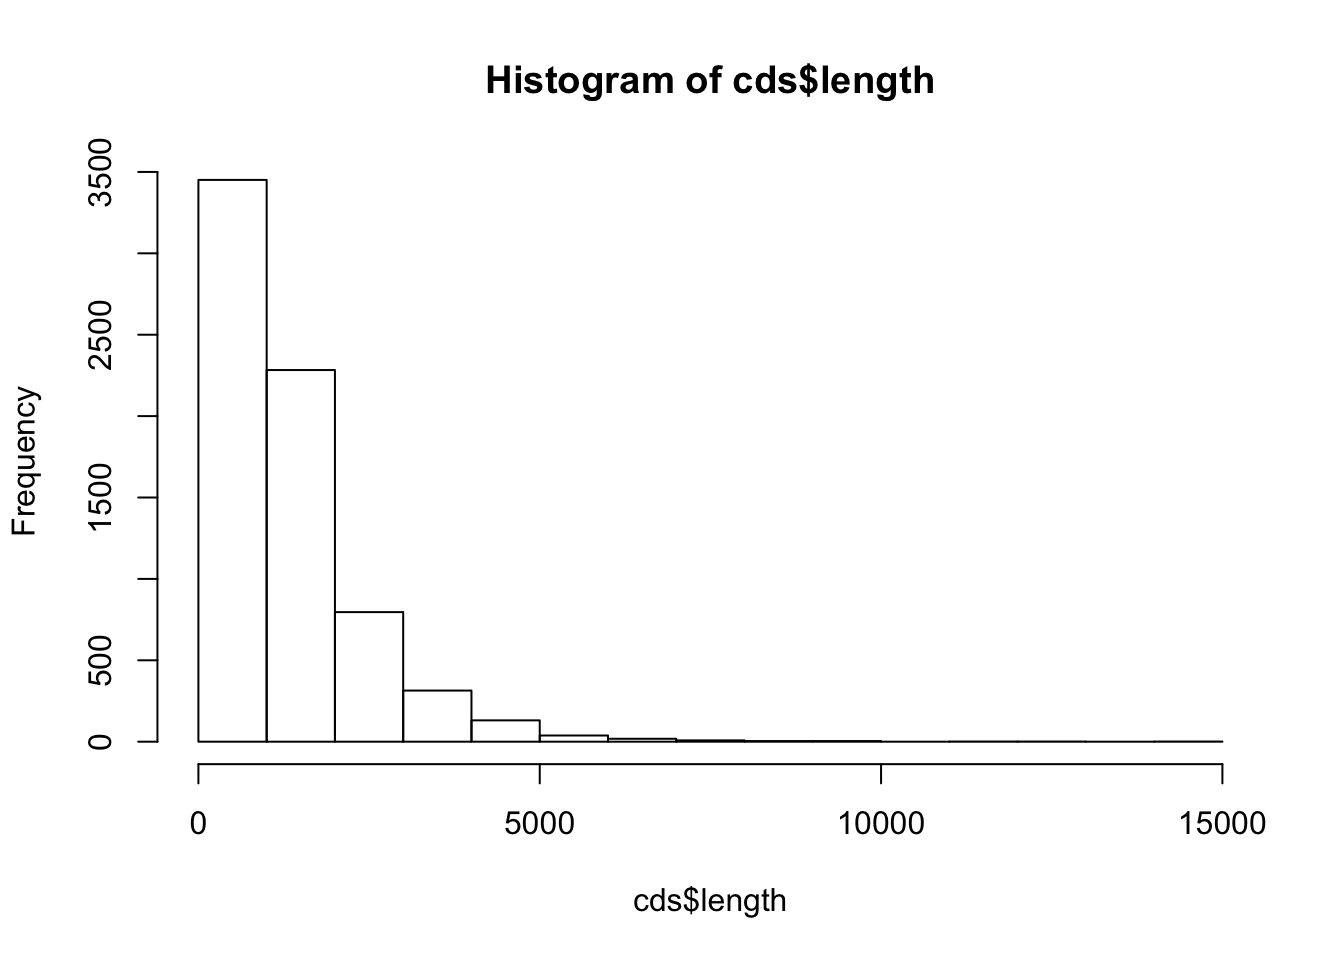
\includegraphics{figures/unnamed-chunk-20-1} \end{center}

Choose the class intervals in a way that the histogram is informative
(neither too large nor too few classes).

\begin{Shaded}
\begin{Highlighting}[]
\NormalTok{## Take more or less 100 bins}
\NormalTok{h <-}\StringTok{ }\KeywordTok{hist}\NormalTok{(cds}\OperatorTok{$}\NormalTok{length, }\DataTypeTok{breaks=}\DecValTok{100}\NormalTok{)}
\end{Highlighting}
\end{Shaded}

\begin{center}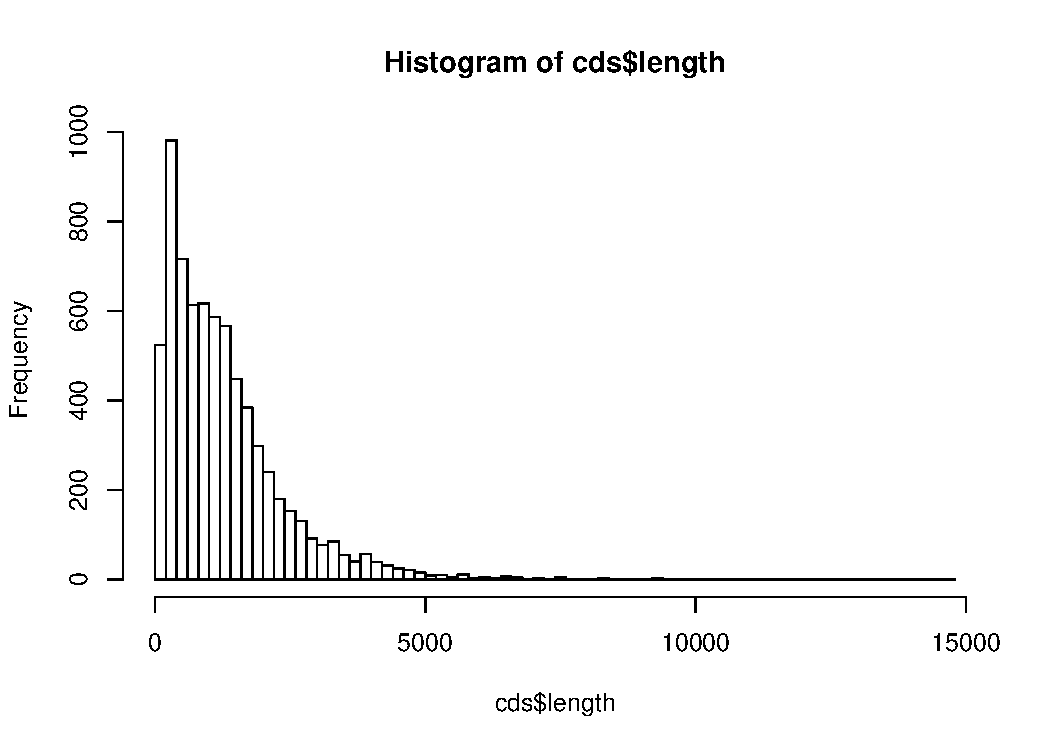
\includegraphics{figures/unnamed-chunk-21-1} \end{center}

Retrieve the result of \texttt{hist()} in a variable named
\texttt{cds.length.hist}.

\begin{Shaded}
\begin{Highlighting}[]
\NormalTok{## Define breaks exactly in the way you wish}
\NormalTok{cds.length.hist <-}\StringTok{ }\KeywordTok{hist}\NormalTok{(cds}\OperatorTok{$}\NormalTok{length, }\DataTypeTok{breaks=}\KeywordTok{seq}\NormalTok{(}\DataTypeTok{from=}\DecValTok{0}\NormalTok{, }\DataTypeTok{to=}\KeywordTok{max}\NormalTok{(cds}\OperatorTok{$}\NormalTok{length)}\OperatorTok{+}\DecValTok{100}\NormalTok{, }\DataTypeTok{by=}\DecValTok{100}\NormalTok{))}
\end{Highlighting}
\end{Shaded}

\begin{center}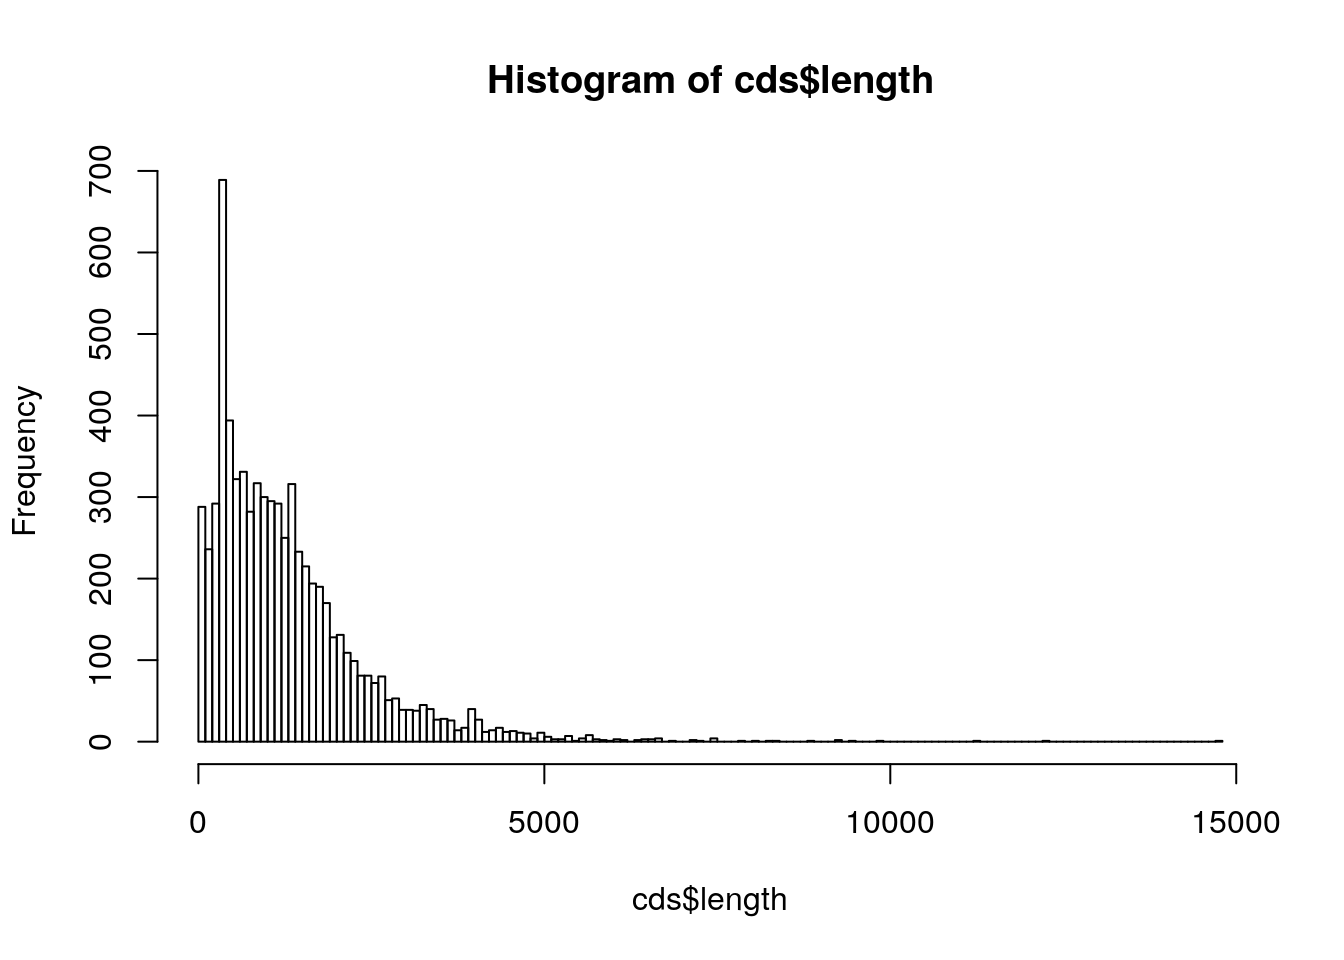
\includegraphics{figures/unnamed-chunk-22-1} \end{center}

Print the result on the screen (\texttt{print()}) and analyze the
structure of the variable \texttt{cds.length.hist} (this is a list
variable).

Useful functions:

\begin{Shaded}
\begin{Highlighting}[]
\NormalTok{## Display the values used to draw the histogram}
\KeywordTok{print}\NormalTok{(cds.length.hist )}
\end{Highlighting}
\end{Shaded}

\begin{verbatim}
$breaks
  [1]     0   100   200   300   400   500   600   700   800   900  1000
 [12]  1100  1200  1300  1400  1500  1600  1700  1800  1900  2000  2100
 [23]  2200  2300  2400  2500  2600  2700  2800  2900  3000  3100  3200
 [34]  3300  3400  3500  3600  3700  3800  3900  4000  4100  4200  4300
 [45]  4400  4500  4600  4700  4800  4900  5000  5100  5200  5300  5400
 [56]  5500  5600  5700  5800  5900  6000  6100  6200  6300  6400  6500
 [67]  6600  6700  6800  6900  7000  7100  7200  7300  7400  7500  7600
 [78]  7700  7800  7900  8000  8100  8200  8300  8400  8500  8600  8700
 [89]  8800  8900  9000  9100  9200  9300  9400  9500  9600  9700  9800
[100]  9900 10000 10100 10200 10300 10400 10500 10600 10700 10800 10900
[111] 11000 11100 11200 11300 11400 11500 11600 11700 11800 11900 12000
[122] 12100 12200 12300 12400 12500 12600 12700 12800 12900 13000 13100
[133] 13200 13300 13400 13500 13600 13700 13800 13900 14000 14100 14200
[144] 14300 14400 14500 14600 14700 14800

$counts
  [1] 288 236 292 689 394 322 331 282 317 300 295 292 250 316 233 215 194
 [18] 190 170 128 131 109  99  81  81  72  80  51  53  39  39  38  45  40
 [35]  27  28  26  14  17  40  27  12  14  17  12  13  11  10   4  11   6
 [52]   3   3   7   1   4   8   3   2   1   3   2   0   2   3   3   4   0
 [69]   1   0   0   2   1   0   4   0   0   0   1   0   1   0   1   1   0
 [86]   0   0   0   1   0   0   0   2   0   1   0   0   0   1   0   0   0
[103]   0   0   0   0   0   0   0   0   0   0   1   0   0   0   0   0   0
[120]   0   0   0   1   0   0   0   0   0   0   0   0   0   0   0   0   0
[137]   0   0   0   0   0   0   0   0   0   0   0   1

$density
  [1] 4.085106e-04 3.347518e-04 4.141844e-04 9.773050e-04 5.588652e-04
  [6] 4.567376e-04 4.695035e-04 4.000000e-04 4.496454e-04 4.255319e-04
 [11] 4.184397e-04 4.141844e-04 3.546099e-04 4.482270e-04 3.304965e-04
 [16] 3.049645e-04 2.751773e-04 2.695035e-04 2.411348e-04 1.815603e-04
 [21] 1.858156e-04 1.546099e-04 1.404255e-04 1.148936e-04 1.148936e-04
 [26] 1.021277e-04 1.134752e-04 7.234043e-05 7.517730e-05 5.531915e-05
 [31] 5.531915e-05 5.390071e-05 6.382979e-05 5.673759e-05 3.829787e-05
 [36] 3.971631e-05 3.687943e-05 1.985816e-05 2.411348e-05 5.673759e-05
 [41] 3.829787e-05 1.702128e-05 1.985816e-05 2.411348e-05 1.702128e-05
 [46] 1.843972e-05 1.560284e-05 1.418440e-05 5.673759e-06 1.560284e-05
 [51] 8.510638e-06 4.255319e-06 4.255319e-06 9.929078e-06 1.418440e-06
 [56] 5.673759e-06 1.134752e-05 4.255319e-06 2.836879e-06 1.418440e-06
 [61] 4.255319e-06 2.836879e-06 0.000000e+00 2.836879e-06 4.255319e-06
 [66] 4.255319e-06 5.673759e-06 0.000000e+00 1.418440e-06 0.000000e+00
 [71] 0.000000e+00 2.836879e-06 1.418440e-06 0.000000e+00 5.673759e-06
 [76] 0.000000e+00 0.000000e+00 0.000000e+00 1.418440e-06 0.000000e+00
 [81] 1.418440e-06 0.000000e+00 1.418440e-06 1.418440e-06 0.000000e+00
 [86] 0.000000e+00 0.000000e+00 0.000000e+00 1.418440e-06 0.000000e+00
 [91] 0.000000e+00 0.000000e+00 2.836879e-06 0.000000e+00 1.418440e-06
 [96] 0.000000e+00 0.000000e+00 0.000000e+00 1.418440e-06 0.000000e+00
[101] 0.000000e+00 0.000000e+00 0.000000e+00 0.000000e+00 0.000000e+00
[106] 0.000000e+00 0.000000e+00 0.000000e+00 0.000000e+00 0.000000e+00
[111] 0.000000e+00 0.000000e+00 1.418440e-06 0.000000e+00 0.000000e+00
[116] 0.000000e+00 0.000000e+00 0.000000e+00 0.000000e+00 0.000000e+00
[121] 0.000000e+00 0.000000e+00 1.418440e-06 0.000000e+00 0.000000e+00
[126] 0.000000e+00 0.000000e+00 0.000000e+00 0.000000e+00 0.000000e+00
[131] 0.000000e+00 0.000000e+00 0.000000e+00 0.000000e+00 0.000000e+00
[136] 0.000000e+00 0.000000e+00 0.000000e+00 0.000000e+00 0.000000e+00
[141] 0.000000e+00 0.000000e+00 0.000000e+00 0.000000e+00 0.000000e+00
[146] 0.000000e+00 0.000000e+00 1.418440e-06

$mids
  [1]    50   150   250   350   450   550   650   750   850   950  1050
 [12]  1150  1250  1350  1450  1550  1650  1750  1850  1950  2050  2150
 [23]  2250  2350  2450  2550  2650  2750  2850  2950  3050  3150  3250
 [34]  3350  3450  3550  3650  3750  3850  3950  4050  4150  4250  4350
 [45]  4450  4550  4650  4750  4850  4950  5050  5150  5250  5350  5450
 [56]  5550  5650  5750  5850  5950  6050  6150  6250  6350  6450  6550
 [67]  6650  6750  6850  6950  7050  7150  7250  7350  7450  7550  7650
 [78]  7750  7850  7950  8050  8150  8250  8350  8450  8550  8650  8750
 [89]  8850  8950  9050  9150  9250  9350  9450  9550  9650  9750  9850
[100]  9950 10050 10150 10250 10350 10450 10550 10650 10750 10850 10950
[111] 11050 11150 11250 11350 11450 11550 11650 11750 11850 11950 12050
[122] 12150 12250 12350 12450 12550 12650 12750 12850 12950 13050 13150
[133] 13250 13350 13450 13550 13650 13750 13850 13950 14050 14150 14250
[144] 14350 14450 14550 14650 14750

$xname
[1] "cds$length"

$equidist
[1] TRUE

attr(,"class")
[1] "histogram"
\end{verbatim}

\begin{itemize}
\tightlist
\item
  \texttt{class(cds.length.hist)}
\item
  \texttt{attributes(cds.length.hist)}
\end{itemize}

Other types of graphs allow you to explore the distribution of a set of
data. In particular, box plots display, for a series of data, the
median, the interquartile range, a confidence interval and outliers.

\begin{Shaded}
\begin{Highlighting}[]
\KeywordTok{boxplot}\NormalTok{(length }\OperatorTok{~}\StringTok{ }\NormalTok{seqname, }\DataTypeTok{data =}\NormalTok{ cds, }\DataTypeTok{col=}\StringTok{"palegreen"}\NormalTok{, }\DataTypeTok{horizontal=}\OtherTok{TRUE}\NormalTok{, }\DataTypeTok{las=}\DecValTok{1}\NormalTok{, }\DataTypeTok{xlab=}\StringTok{"Gene length"}\NormalTok{, }\DataTypeTok{ylab=}\StringTok{"Chromosome"}\NormalTok{)}
\end{Highlighting}
\end{Shaded}

\begin{figure}

{\centering 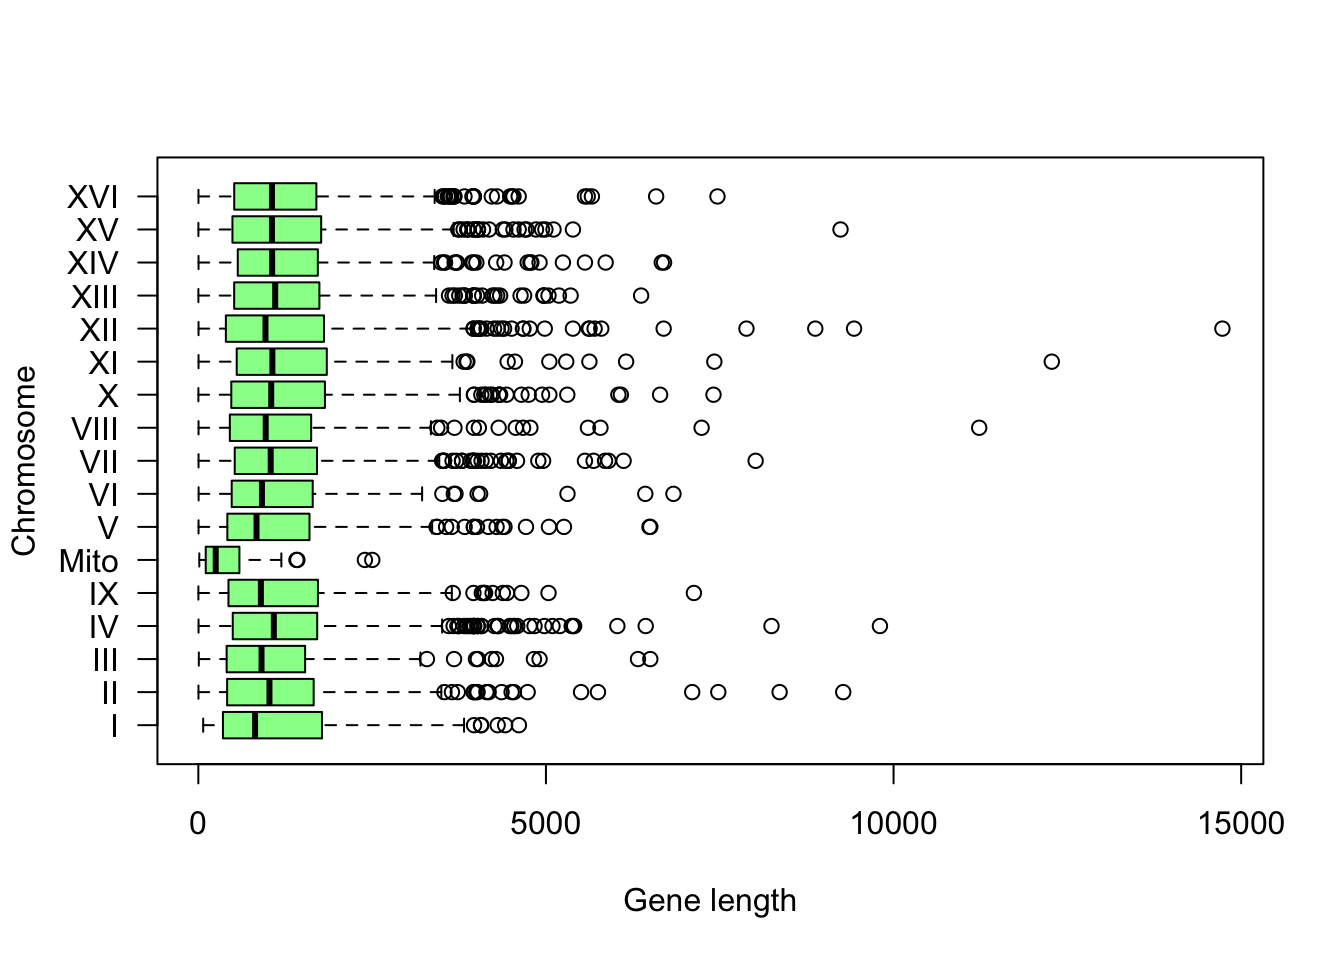
\includegraphics{figures/unnamed-chunk-24-1} 

}

\caption{Boîte à moustache indiquant la distribution de longueur des gènes par chromosome. }\label{fig:unnamed-chunk-24}
\end{figure}

\subsubsection{7. Descriptive parameters}\label{descriptive-parameters}

Calculate the parameters of central tendency (mean, median, mode) and
dispersion (variance, standard deviation, inter-quartile deviation)

\begin{itemize}
\tightlist
\item
  for the genes of chromosome III;
\item
  for all yeast genes.
\end{itemize}

\begin{Shaded}
\begin{Highlighting}[]
\NormalTok{x <-}\StringTok{ }\KeywordTok{subset}\NormalTok{(cds, seqname }\OperatorTok{==}\StringTok{ "III"}\NormalTok{, }\DataTypeTok{select =} \StringTok{"length"}\NormalTok{)}
\KeywordTok{dim}\NormalTok{(x) }
\end{Highlighting}
\end{Shaded}

\begin{verbatim}
[1] 194   1
\end{verbatim}

\begin{Shaded}
\begin{Highlighting}[]
\KeywordTok{class}\NormalTok{(x) ## Ah ah, this is not a vector but a data.frame}
\end{Highlighting}
\end{Shaded}

\begin{verbatim}
[1] "data.frame"
\end{verbatim}

\begin{Shaded}
\begin{Highlighting}[]
\NormalTok{## Convert the data frame into a vector}
\NormalTok{x <-}\StringTok{ }\KeywordTok{unlist}\NormalTok{(x)}
\KeywordTok{class}\NormalTok{(x)}
\end{Highlighting}
\end{Shaded}

\begin{verbatim}
[1] "numeric"
\end{verbatim}

\begin{Shaded}
\begin{Highlighting}[]
\KeywordTok{head}\NormalTok{(x)}
\end{Highlighting}
\end{Shaded}

\begin{verbatim}
length1 length2 length3 length4 length5 length6 
    741    1845    1374     780     630     525 
\end{verbatim}

\begin{Shaded}
\begin{Highlighting}[]
\NormalTok{## Compute the mean, either manually or with the ad hoc R function}
\NormalTok{n <-}\StringTok{ }\KeywordTok{length}\NormalTok{(x) }
\KeywordTok{print}\NormalTok{(}\KeywordTok{paste}\NormalTok{(}\StringTok{"Chromosome III contains"}\NormalTok{, n, }\StringTok{"CDS"}\NormalTok{))}
\end{Highlighting}
\end{Shaded}

\begin{verbatim}
[1] "Chromosome III contains 194 CDS"
\end{verbatim}

\begin{Shaded}
\begin{Highlighting}[]
\KeywordTok{message}\NormalTok{(}\StringTok{"Chromosome III contains "}\NormalTok{, n, }\StringTok{" CDS"}\NormalTok{)}

\NormalTok{m <-}\StringTok{ }\KeywordTok{mean}\NormalTok{(x)}
\KeywordTok{print}\NormalTok{(m)}
\end{Highlighting}
\end{Shaded}

\begin{verbatim}
[1] 1169.521
\end{verbatim}

\begin{Shaded}
\begin{Highlighting}[]
\KeywordTok{message}\NormalTok{(}\StringTok{"mean(x) = "}\NormalTok{, }\KeywordTok{round}\NormalTok{(m, }\DataTypeTok{digits =} \DecValTok{1}\NormalTok{))}

\NormalTok{## Compute the mean manually to compare the result}
\NormalTok{m.recalc <-}\StringTok{ }\KeywordTok{sum}\NormalTok{(x)}\OperatorTok{/}\NormalTok{n}
\KeywordTok{message}\NormalTok{(}\StringTok{"Manually computed sample mean: "}\NormalTok{, }\KeywordTok{round}\NormalTok{(}\DataTypeTok{digits=}\DecValTok{1}\NormalTok{, m.recalc))}

\NormalTok{## Compute manually standard dev of the sample}
\NormalTok{sample.var <-}\StringTok{ }\KeywordTok{sum}\NormalTok{((x }\OperatorTok{-}\StringTok{ }\NormalTok{m)}\OperatorTok{^}\DecValTok{2}\NormalTok{)}\OperatorTok{/}\StringTok{ }\NormalTok{n}
\NormalTok{sample.sd <-}\StringTok{ }\KeywordTok{sqrt}\NormalTok{(sample.var)}
\KeywordTok{message}\NormalTok{(}\StringTok{"Sample standard dev ="}\NormalTok{, }\KeywordTok{round}\NormalTok{(}\DataTypeTok{digits=}\DecValTok{1}\NormalTok{, sample.sd))}

\NormalTok{## Compute an estimate of the population standard deviation}
\NormalTok{pop.sd.est <-}\StringTok{ }\KeywordTok{sqrt}\NormalTok{(}\KeywordTok{sum}\NormalTok{((x }\OperatorTok{-}\StringTok{ }\NormalTok{m)}\OperatorTok{^}\DecValTok{2}\NormalTok{) }\OperatorTok{/}\StringTok{ }\NormalTok{(n}\OperatorTok{-}\DecValTok{1}\NormalTok{))}
\KeywordTok{message}\NormalTok{(}\StringTok{"Sample-based estimate of population standard dev ="}\NormalTok{, }\KeywordTok{round}\NormalTok{(}\DataTypeTok{digits=}\DecValTok{1}\NormalTok{, pop.sd.est))}

\NormalTok{## Compute the standard deviation with R function sd()}
\NormalTok{R.sd <-}\StringTok{ }\KeywordTok{sd}\NormalTok{(x)}
\KeywordTok{message}\NormalTok{(}\StringTok{"Result of R sd() function ="}\NormalTok{, }\KeywordTok{round}\NormalTok{(}\DataTypeTok{digits=}\DecValTok{1}\NormalTok{, R.sd))}
\end{Highlighting}
\end{Shaded}

\textbf{Ah ah! (skeptical tone)} The R function \texttt{sd()} does
\textbf{not} compute the standard deviation of the input numbers
(\(s\)), but the \textbf{estimate of the standard deviaiton of the
population} (\(\hat{\sigma}\))

Display these parameters on the histogram of gene length, using the
function \texttt{arrows()}

\subsubsection{8. Intervalle de
confiance}\label{intervalle-de-confiance}

From genes of chromosome III (considered as the sample available in
1992), calculate a confidence interval around the mean, and formulate
the interpretation of this confidence interval. Then evaluate whether or
not this confidence interval covered the average population (all genes
in the yeast genome, which became available 4 years after chromosome
III).

\[ \bar{x} \pm \frac{\hat{\sigma}}{\sqrt(n)} \cdot t_{1-\alpha/2}^{n-1}\]

\begin{Shaded}
\begin{Highlighting}[]
\NormalTok{## Define alpha, the risk}
\NormalTok{alpha <-}\StringTok{ }\FloatTok{0.05}

\NormalTok{## Let us get the critical value for the t distribution}
\KeywordTok{help}\NormalTok{(}\StringTok{"TDist"}\NormalTok{)}

\NormalTok{## Which value corresponds to alpha/2 }

\NormalTok{## Beware ! by default the qt() function return the lower tail}
\KeywordTok{qt}\NormalTok{(}\DataTypeTok{p =}\NormalTok{ alpha}\OperatorTok{/}\DecValTok{2}\NormalTok{, }\DataTypeTok{df =}\NormalTok{  n }\OperatorTok{-}\StringTok{ }\DecValTok{1}\NormalTok{)}
\end{Highlighting}
\end{Shaded}

\begin{verbatim}
[1] -1.972332
\end{verbatim}

\begin{Shaded}
\begin{Highlighting}[]
\NormalTok{## For confidence intervals we need a positive t value, we thus take the upper tail}
\NormalTok{t.value <-}\StringTok{ }\KeywordTok{qt}\NormalTok{(}\DataTypeTok{p =}\NormalTok{ alpha}\OperatorTok{/}\DecValTok{2}\NormalTok{, }\DataTypeTok{df =}\NormalTok{  n }\OperatorTok{-}\StringTok{ }\DecValTok{1}\NormalTok{, }\DataTypeTok{lower.tail =} \OtherTok{FALSE}\NormalTok{)}

\NormalTok{IC.min <-}\StringTok{ }\NormalTok{m }\OperatorTok{-}\StringTok{ }\NormalTok{pop.sd.est }\OperatorTok{*}\StringTok{ }\NormalTok{t.value }\OperatorTok{/}\KeywordTok{sqrt}\NormalTok{(n)}
\NormalTok{IC.max <-}\StringTok{ }\NormalTok{m }\OperatorTok{+}\StringTok{ }\NormalTok{pop.sd.est }\OperatorTok{*}\StringTok{ }\NormalTok{t.value }\OperatorTok{/}\KeywordTok{sqrt}\NormalTok{(n)}

\KeywordTok{message}\NormalTok{(}\StringTok{"Confidence interval: ["}\NormalTok{, }
        \KeywordTok{round}\NormalTok{(}\DataTypeTok{digits=}\DecValTok{1}\NormalTok{, IC.min), }
        \StringTok{", "}\NormalTok{, }
        \KeywordTok{round}\NormalTok{(}\DataTypeTok{digits=}\DecValTok{1}\NormalTok{, IC.max), }\StringTok{"]"}\NormalTok{)}
\end{Highlighting}
\end{Shaded}

Draw a polygnone of frequencies indicating the number of genes per class
(class medium).

\begin{Shaded}
\begin{Highlighting}[]
\NormalTok{## Draw a frequency polygon}
\KeywordTok{plot}\NormalTok{(cds.length.hist }\OperatorTok{$}\NormalTok{mids, cds.length.hist }\OperatorTok{$}\NormalTok{counts, }
     \DataTypeTok{main=}\StringTok{"Frequency polygon"}\NormalTok{, }
     \DataTypeTok{xlab=}\StringTok{"Gene length"}\NormalTok{, }\DataTypeTok{ylab=}\StringTok{"Number of genes"}\NormalTok{, }
     \DataTypeTok{type=}\StringTok{"l"}\NormalTok{, }\DataTypeTok{col=}\StringTok{"darkgreen"}\NormalTok{, }\DataTypeTok{lwd=}\DecValTok{2}\NormalTok{, }\DataTypeTok{xlim=}\KeywordTok{c}\NormalTok{(}\DecValTok{0}\NormalTok{, }\DecValTok{5000}\NormalTok{))}
\KeywordTok{grid}\NormalTok{()}

\KeywordTok{arrows}\NormalTok{(}\DataTypeTok{x0 =}\NormalTok{ IC.min, }\DataTypeTok{y0 =} \DecValTok{100}\NormalTok{, }\DataTypeTok{x1 =}\NormalTok{ IC.max, }\DataTypeTok{y1=}\DecValTok{100}\NormalTok{, }\DataTypeTok{length =} \DecValTok{0}\NormalTok{, }\DataTypeTok{angle =} \DecValTok{00}\NormalTok{, }\DataTypeTok{col=}\StringTok{"violet"}\NormalTok{, }\DataTypeTok{lwd=}\DecValTok{3}\NormalTok{)}
\KeywordTok{abline}\NormalTok{(}\DataTypeTok{v =}\NormalTok{ m, }\DataTypeTok{col=}\StringTok{"violet"}\NormalTok{)}

\NormalTok{pop.mean <-}\StringTok{ }\KeywordTok{mean}\NormalTok{(cds}\OperatorTok{$}\NormalTok{length)}
\KeywordTok{abline}\NormalTok{(}\DataTypeTok{v =}\NormalTok{ pop.mean, }\DataTypeTok{col=}\StringTok{"blue"}\NormalTok{)}

\KeywordTok{legend}\NormalTok{(}\StringTok{"topright"}\NormalTok{, }\DataTypeTok{legend =} \KeywordTok{c}\NormalTok{(}\StringTok{"genome"}\NormalTok{, }\StringTok{"chr3"}\NormalTok{), }\DataTypeTok{col =} \KeywordTok{c}\NormalTok{(}\StringTok{"blue"}\NormalTok{, }\StringTok{"violet"}\NormalTok{), }\DataTypeTok{lwd=}\DecValTok{1}\NormalTok{)}
\end{Highlighting}
\end{Shaded}

\begin{center}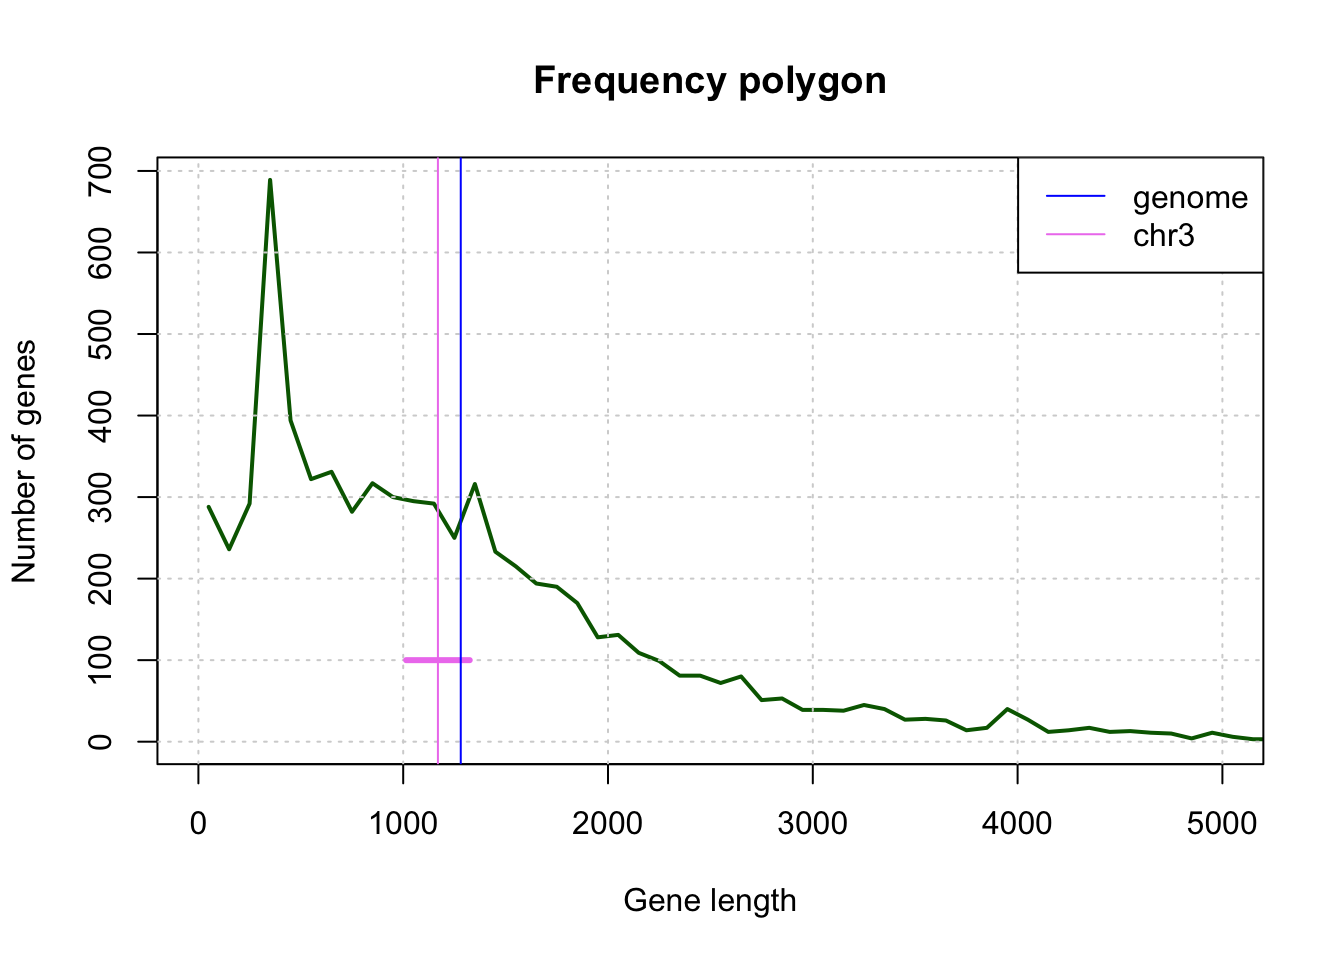
\includegraphics{figures/unnamed-chunk-27-1} \end{center}

\subsubsection{9. Distribution of gene
length}\label{distribution-of-gene-length}

\begin{itemize}
\item
  From the result of \texttt{hist()}, retrieve an array (in a variable
  of type \texttt{data.frame}) indicating the absolute frequencies
  (\texttt{count}) according to the median class size (\texttt{mids}),
\item
  Add to this table a column indicating the relative frequency of each
  class of gene length.
\item
  Add columns to this table indicating the \textbf{empirical
  distribution function} gene lengths (number of genes of a size less
  than or equal to each observed \(x\) value, and relative frequency of
  this number).

  \begin{itemize}
  \tightlist
  \item
    basic function: \texttt{cumsum()}
  \item
    advanced function:\texttt{ecdf()}
  \end{itemize}
\item
  by using the functions \texttt{plot()} and \texttt{lines()}, draw a
  graph representing the absolute frequency per class (medians of
  classes in \(X\), counts in \(Y\)), and the empirical distribution
  function.

  \begin{itemize}
  \tightlist
  \item
    suggestion: superposez les ??utilisez le type de lignes ``h'' pour
    les fréquences de classe, et ``l'' ou ``s'' pour la fonction de
    répartition.
  \end{itemize}
\end{itemize}

\subsubsection{10. Randomly expected distribution for gene
length}\label{randomly-expected-distribution-for-gene-length}

Based on the genome size (12.156.679 bp) and codon genomic frequencies
defined below, calculate the random expected gene length distribution,
and add it to the graph.

You can download the genomic frequencies of all trinucleotides here:
\href{http://jvanheld.github.io/stat1/data/Saccharomyces_cerevisiae/oligo_freq/3nt_genomic_Saccharomyces_cerevisiae-ovlp-1str.tab}{3nt\_genomic\_Saccharomyces\_cerevisiae-ovlp-1str.tab}

Alternative: create a variable \texttt{freq.3nt} and manually assign the
values for the 4? required nucleotides from the table below.

\begin{longtable}[]{@{}lrr@{}}
\toprule
sequence & frequency & occurrences\tabularnewline
\midrule
\endhead
AAA & 0.0394 & 478708\tabularnewline
ATG & 0.0183 & 221902\tabularnewline
TAA & 0.0224 & 272041\tabularnewline
TAG & 0.0129 & 156668\tabularnewline
TGA & 0.0201 & 244627\tabularnewline
\bottomrule
\end{longtable}

\subsubsection{11. Before finishing~: keep track of your
session}\label{before-finishing-keep-track-of-your-session}

Traceability is an essential issue in science. The function
\textbf{\emph{R}} \texttt{sessionInfo()} provides a summary of the
conditions of a work session: version of R, operator system, libraries
of functions used.

\begin{Shaded}
\begin{Highlighting}[]
\KeywordTok{sessionInfo}\NormalTok{()}
\end{Highlighting}
\end{Shaded}

\begin{verbatim}
R version 3.6.1 (2019-07-05)
Platform: x86_64-pc-linux-gnu (64-bit)
Running under: Ubuntu 18.04.2 LTS

Matrix products: default
BLAS:   /usr/lib/x86_64-linux-gnu/blas/libblas.so.3.7.1
LAPACK: /usr/lib/x86_64-linux-gnu/lapack/liblapack.so.3.7.1

locale:
 [1] LC_CTYPE=fr_FR.UTF-8       LC_NUMERIC=C              
 [3] LC_TIME=fr_FR.UTF-8        LC_COLLATE=fr_FR.UTF-8    
 [5] LC_MONETARY=fr_FR.UTF-8    LC_MESSAGES=fr_FR.UTF-8   
 [7] LC_PAPER=fr_FR.UTF-8       LC_NAME=C                 
 [9] LC_ADDRESS=C               LC_TELEPHONE=C            
[11] LC_MEASUREMENT=fr_FR.UTF-8 LC_IDENTIFICATION=C       

attached base packages:
[1] stats     graphics  grDevices utils     datasets  methods   base     

other attached packages:
[1] knitr_1.24

loaded via a namespace (and not attached):
 [1] compiler_3.6.1  magrittr_1.5    tools_3.6.1     htmltools_0.3.6
 [5] yaml_2.2.0      Rcpp_1.0.2      stringi_1.4.3   rmarkdown_1.15 
 [9] highr_0.8       stringr_1.4.0   xfun_0.9        digest_0.6.20  
[13] evaluate_0.14  
\end{verbatim}


\end{document}
